% created by hand
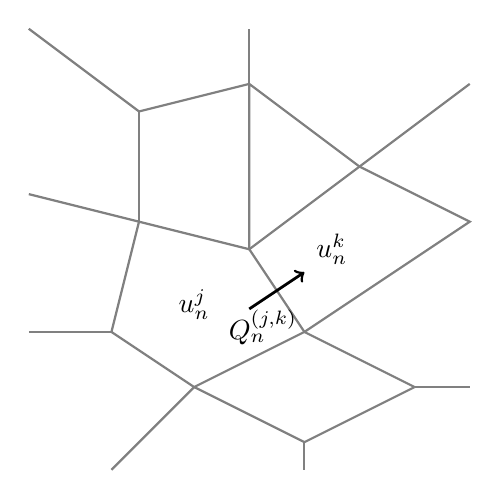
\begin{tikzpicture}[scale=0.35]
  %uncomment to see grid on which it was generated:
  %\draw[dotted,step=1.0,black,very thin] (0,0) grid (16,16);

    % exterior cell boundaries
  \draw[gray, thick] (3,0) -- (6,3);
  \draw[gray, thick] (0,5) -- (3,5);
  \draw[gray, thick] (0,10) -- (4,9);
  \draw[gray, thick] (0,16) -- (4,13);
  \draw[gray, thick] (4,13) -- (4,9);
  \draw[gray, thick] (4,13) -- (8,14);
  \draw[gray, thick] (8,14) -- (8,16);
  \draw[gray, thick] (12,11) -- (16,14);
  \draw[gray, thick] (10,5) -- (14,3);
  \draw[gray, thick] (10,1) -- (14,3);
  \draw[gray, thick] (14,3) -- (16,3);
  \draw[gray, thick] (6,3) -- (10,1);
  \draw[gray, thick] (10,0) -- (10,1);
  % interior cell boundaries
  \draw[gray, thick] (10,5) -- (8,8);
  \draw[gray, thick] (8,8) -- (12,11);



  % the free boundary is just like the other edges
  \draw[gray, thick] (6,3) -- (3,5) -- (4,9) -- (8,8) -- (8,14) --
              (12,11) -- (16,9) -- (10,5) -- cycle;
  % label some cell d.o.f.
  \draw (6,6) node {$u_n^j$};
  \draw (11,8) node {$u_n^k$};
  % show normal flux
  \def\xmid{9};
  \def\ymid{6.5};
  \def\dx{3/3};
  \def\dy{2/3};
  \draw[->,line width=1.0pt] (\xmid-\dx,\ymid-\dy) -- (\xmid+\dx,\ymid+\dy); % normal vector
  \draw (\xmid-\dx/2,\ymid-2*\dy) node {$Q_n^{(j,k)}$}; % label as flux
\end{tikzpicture}
